           
%%%%%%%%%%%%%%%%%%%%%%%%%%%%%%%%%%%%%%%%%%%%%%%%%%%%%%%%%%%%%%%%%%%%%%%%%%%%%%%%%%%%%%%%%%%%%%%%
%%%%%%%%%%%%%%%%%%%%%%%%%%%%%%%%%%%%%%%%%%%%%%%%%%%%%%%%%%%%%%%%%%%%%%%%%%%%%%%%%%%%%%%%%%%%%%%%
\section{Integralrechnung \formelbuch{492}}
\subsection{Integrationsmethoden \formelbuch{495ff}}
\renewcommand{\arraystretch}{2}
\begin{tabular}{| l | l |}
	\hline
		Linearität &
			$\int{f(\alpha x+\beta )dx=\frac{1}{\alpha}\cdot F(\alpha x+\beta)+C}$ \\
	\hline
		Partielle Integration &
			$\int\limits_a^b{u'(x)\cdot v(x)dx}=\biggl[ u(x)\cdot v(x) \biggr]_a^b-\int\limits_a^b{u(x)\cdot v'(x)dx}$ \\
	\hline
		Weierstrass-Substitution &
			$t=\tan\frac{x}{2}, \qquad dx=\frac{2dt}{1+t^2}$
			$\qquad \sin  x=\frac{2t}{1+t^2}$
			$\qquad \cos x=\frac{1-t^2}{1+t^2} \quad\int{R(\sin(x),\cos(x))dx}$ \\
	\hline
		Allgemeine Substitution &
			$\int\limits_{a}^{b}{f(x)dx}=\int\limits_{g^{-1}(a)}^{g^{-1}(b)}{f(g(t))\cdot g'(t)dt}$
			$\qquad t=g^{-1}(x)$
			$\qquad  \fbox{x=g(t)}\Leftrightarrow^{d(...)} dx=g'(t)\cdot dt$ \\
	\hline
		Logarithmische Integration &
			$\int{\frac{f'(x)}{f(x)}dx}=\ln|f(x)|+C$
			$\qquad {(f(x)\neq 1)}$
			$\qquad y'(x)\cdot dx = dy \rightarrow$ allg. gültig\\
	\hline
		Potenzregel &
			$\int{f'(x)\cdot (f(x))^{\alpha} dx}=\frac{f(x)^{\alpha +1}}{\alpha+1}+C$
			$\qquad{(\alpha \neq -1)}$ \\
	\hline
		Differentiation &
			$\int \limits ^{b} _{a} {f'(t)dt}=f(b)-f(a)$
			$\qquad \frac{d}{dx} \int \limits ^{x} _{1} {f(t)dt}=f(x)$ \\
	\hline
			Mittelwerte &
				linear: $\frac{1}{b-a} \int\limits ^{b} _{a} {f(x)dx}$
				$\qquad$ quadratisch: $\sqrt{\frac{1}{b-a} \int\limits ^{b} _{a} {\lvert f(x)^2 \rvert dx}}$ \\
	\hline
\end{tabular}
\renewcommand{\arraystretch}{1}


\subsubsection{Einige unbestimmte Integrale \formelbuch{1081ff}} 
 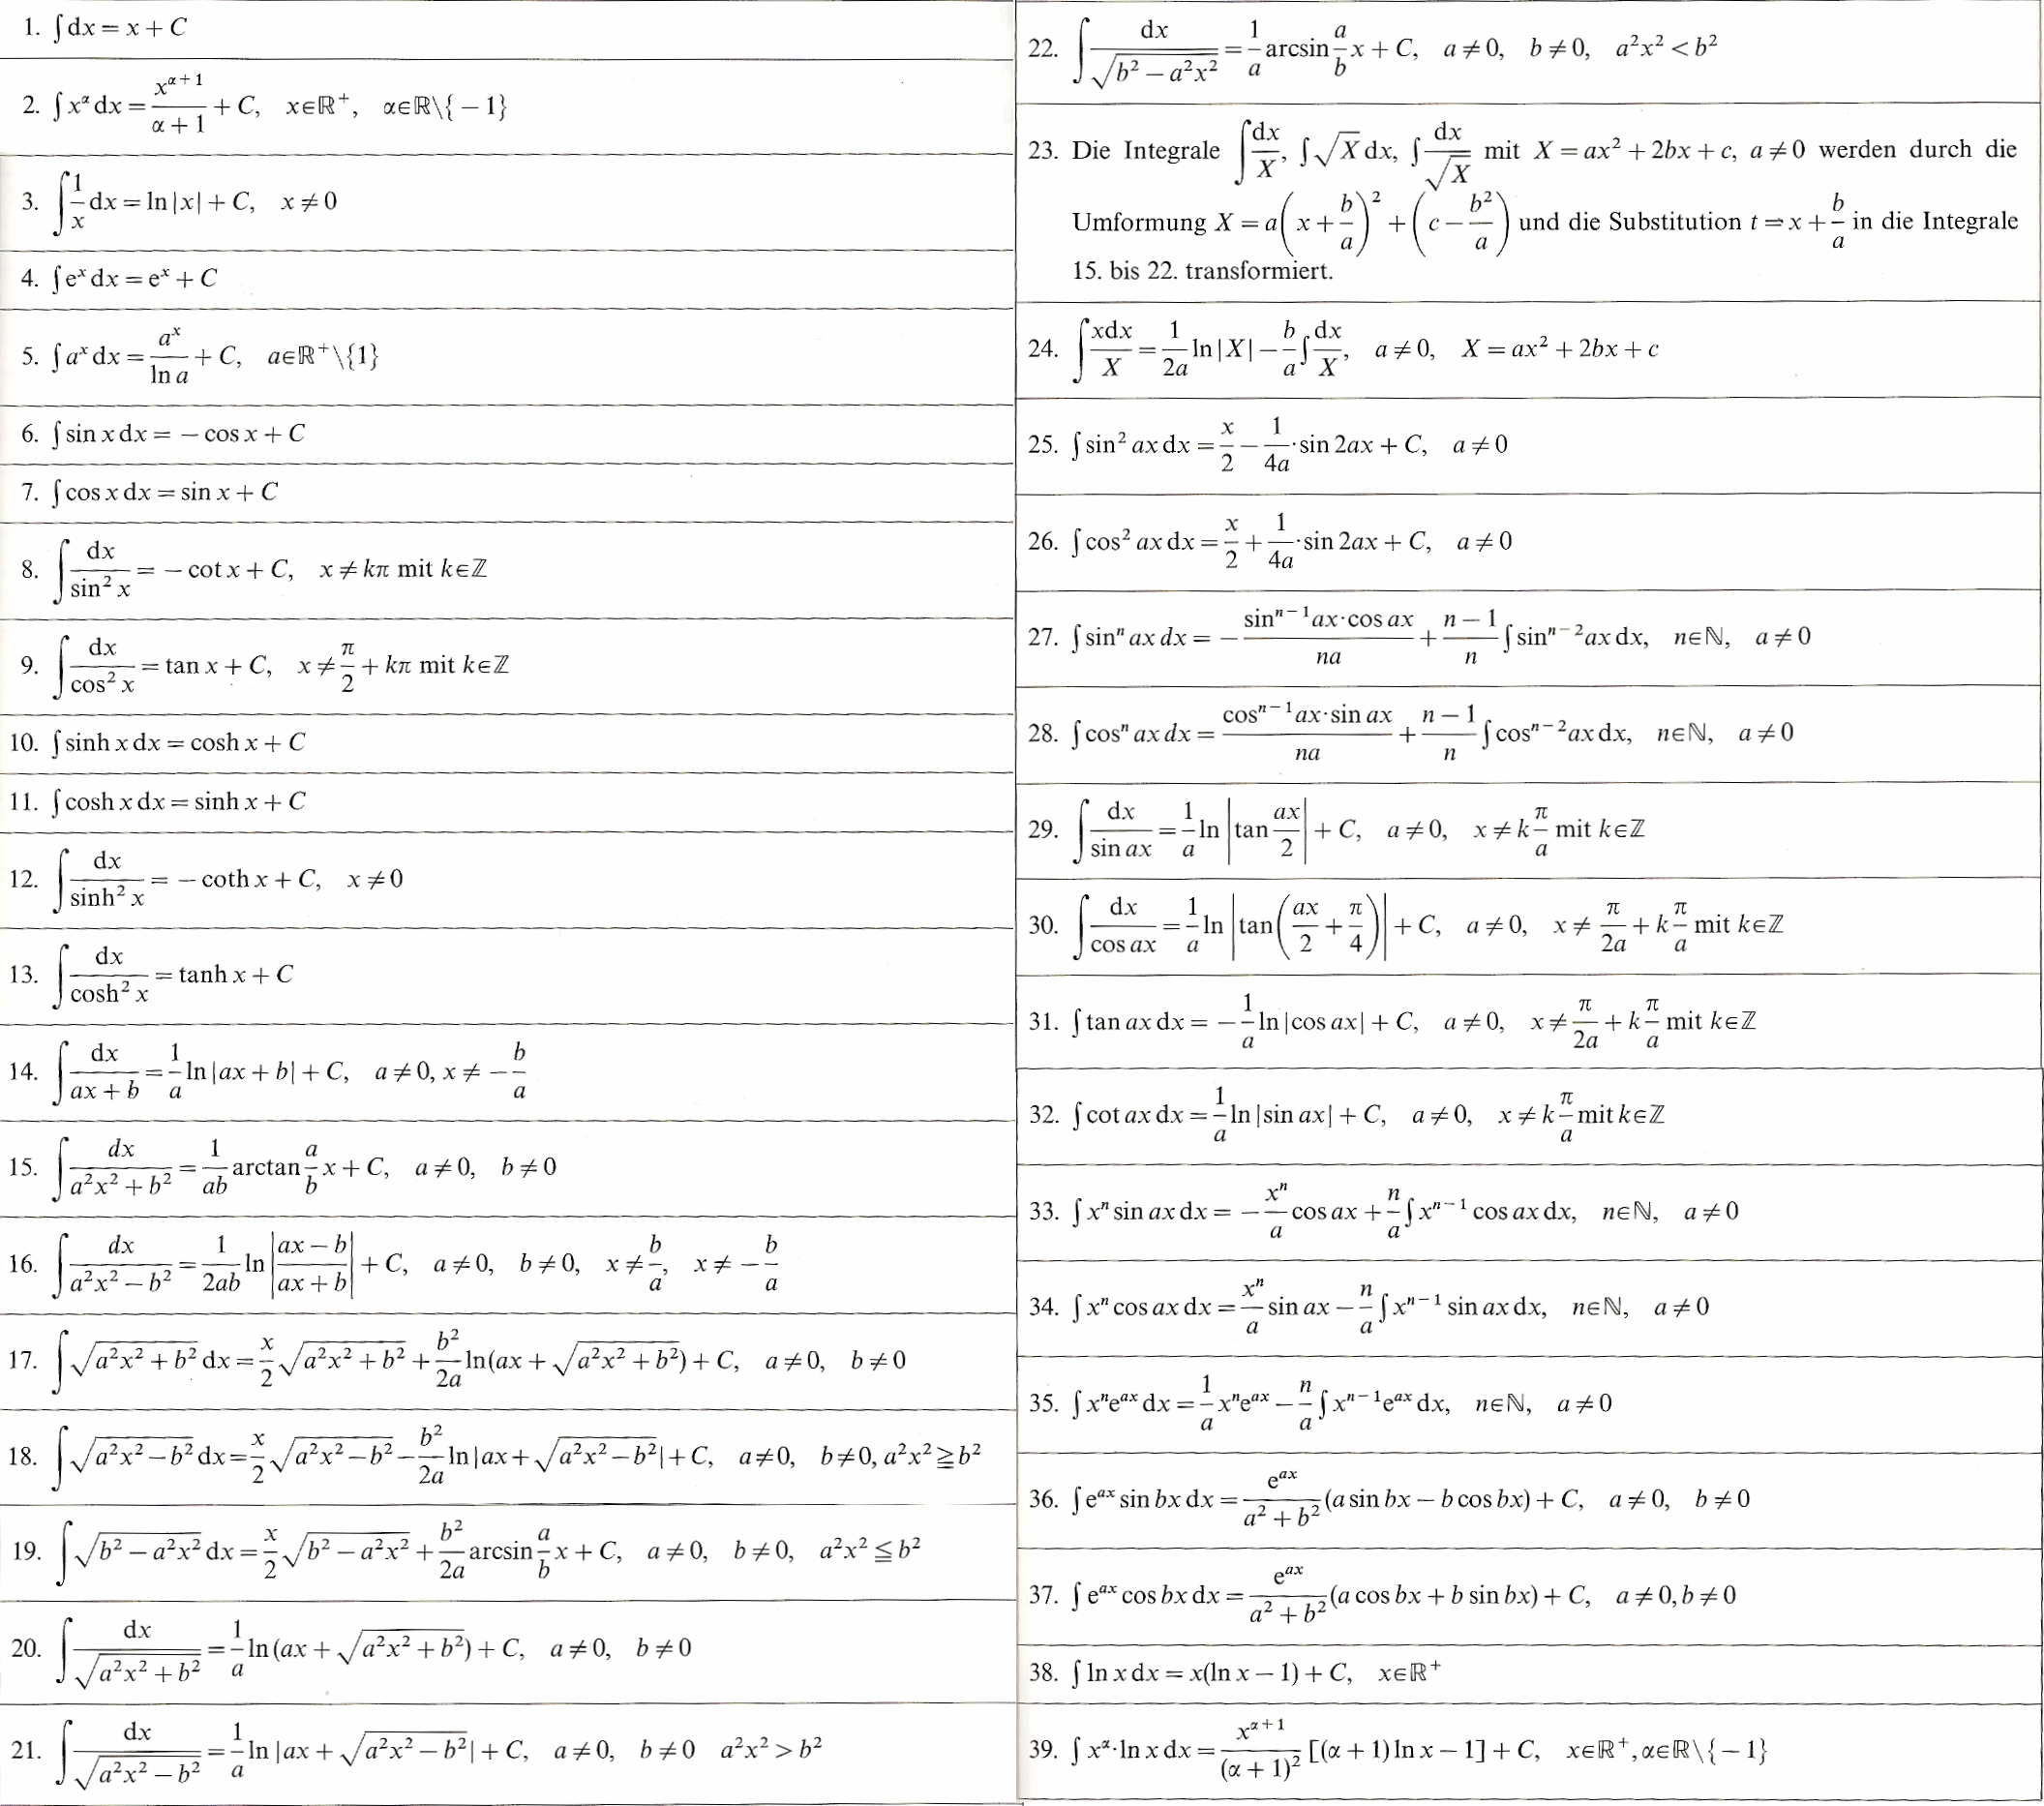
\includegraphics[width=16.1cm]{./bilder/integrale.png} 



\subsection{Uneigentliche Integrale\formelbuch{518}}
	Uneigentliches Integral heisst, dass entweder eine \textbf{unbeschränkte
	Funktion} integriert wird, oder eine Funktion über einen \textbf{unbeschränkten Integrationsberech} 
	integriert wird.$\\$
	\begin{minipage}{100mm}
    
	Für unbeschränkte Funktionen:$\\$
	$I =\int\limits _{a}^{c}f(x)dx=
	\lim\limits_{t\uparrow b}\int\limits_{a}^{t}f(x)dx+\lim\limits_{t\downarrow b}\int\limits_{t}^{c}f(x)dx\\
	\\$ Für die unbeschränkte Integration:$\\$
	$I =\int\limits _{a} ^{\infty} f(x)dx= \lim \limits_{t\to \infty}\int \limits
	_{a} ^{t}f(x)dx;\\$
	$I =\int\limits ^{a} _{-\infty} f(x)dx= \lim \limits_{t\to -\infty}\int
	\limits _{t} ^{a}f(x)dx; \\$
	$I =\int\limits _{-\infty} ^{\infty} f(x)dx = \lim \limits_{t_1\to -\infty} \lim
	\limits
	_{t_2 \to  \infty}\int \limits _{t_1} ^{a}f(x)dx + \int\limits_{a}^{t_2}f(x)dx\\$
	Beispiel: $\int\limits_{1}^{\infty}\frac{1}{x^2}dx=\lim\limits_{t\to \infty}\int\limits_{1}^{t}\frac{1}{x^2}dx=\lim\limits_{t\to \infty}-\frac{1}{t}+\frac{1}{1}=1$
    \end{minipage}
	\begin{minipage}{100mm}
    	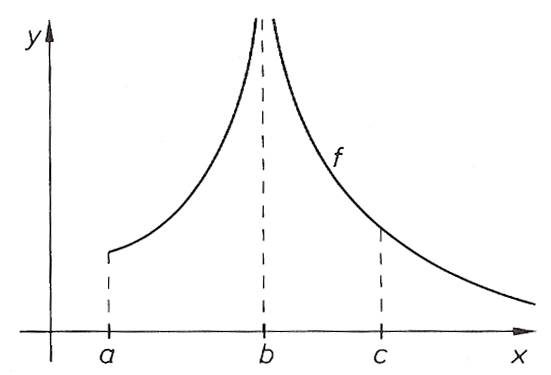
\includegraphics[width=3cm]{./bilder/unbeschraenkteFunktion.png} $\\$
    	unbeschränkte Funktion
    \end{minipage}

\subsubsection{Prinzip der Restfläche}
	Wenn $\lim\limits_{t \rightarrow \infty} \int\limits^{\infty}_{t} f(x) dx = 0$, dann konvergiert
	$\int\limits_a^{\infty} f(x) dx$ und umgekehrt.

\subsubsection{Majorantenprinzip}
	Um nachzuweisen, ob eine Funktion $|f(x)| \geq 0$ absolut konvergiert, wird eine zweite
	Funktion $g(x) \geq |f(x)|$ (Majorante) gesucht. Konvergiert $\int\limits_a^{\infty} g(x) dx$,
	dann konvergiert auch $\int\limits_a^{\infty} |f(x)| dx$ und somit konvergiert auch $\int\limits_a^{\infty} f(x) dx$. $\qquad x \in [a, \infty[$

\subsubsection{Minorantenprinzip}
	Um nachzuweisen, ob eine Funktion $f(x)$ divergiert, wird eine zweite
	Funktion $0 \leq g(x) \leq f(x)$ (Minorante) gesucht. Divergiert
	$\int\limits_a^{\infty} g(x) dx$,
	dann divergiert auch $\int\limits_a^{\infty} f(x) dx$. $\qquad x \in [a, \infty[$
	

%%%%%%%%%%%%%%%%%%%%%%%%%%%%%%%%%%%%%%%%%%%%%%%%%%%%%%%%%%%%%%%%%%%%%%%%%%%%%%%%%%%%%%%%%%%%%%%%
%%%%%%%%%%%%%%%%%%%%%%%%%%%%%%%%%%%%%%%%%%%%%%%%%%%%%%%%%%%%%%%%%%%%%%%%%%%%%%%%%%%%%%%%%%%%%%%%